\documentclass[sigconf]{acmart}

\usepackage{booktabs}
\usepackage{amsmath}

\citestyle{acmauthoryear}
\setcitestyle{square}
\setcopyright{none}

\begin{document}

\title{Implementation of Radiosity}

\author{Sasha Volokh}
\email{sasha.volokh@gmail.com}

\begin{abstract}

This report discusses an implementation of radiosity on top of our previously developed ray tracers. First, the implementation section will detail the core phases and components of the radiosity engine (patch construction, form factor calculation, iterative solving of energy transfer, etc.). Then, the integration of the radiosity engine into the ray tracer will be discussed, and finally some additional enhancements (like material shaders) will be introduced. Lastly, a visual and timing analysis will be done with respect to various parameters of the radiosity engine.

\end{abstract}

\begin{teaserfigure}
  \centering
  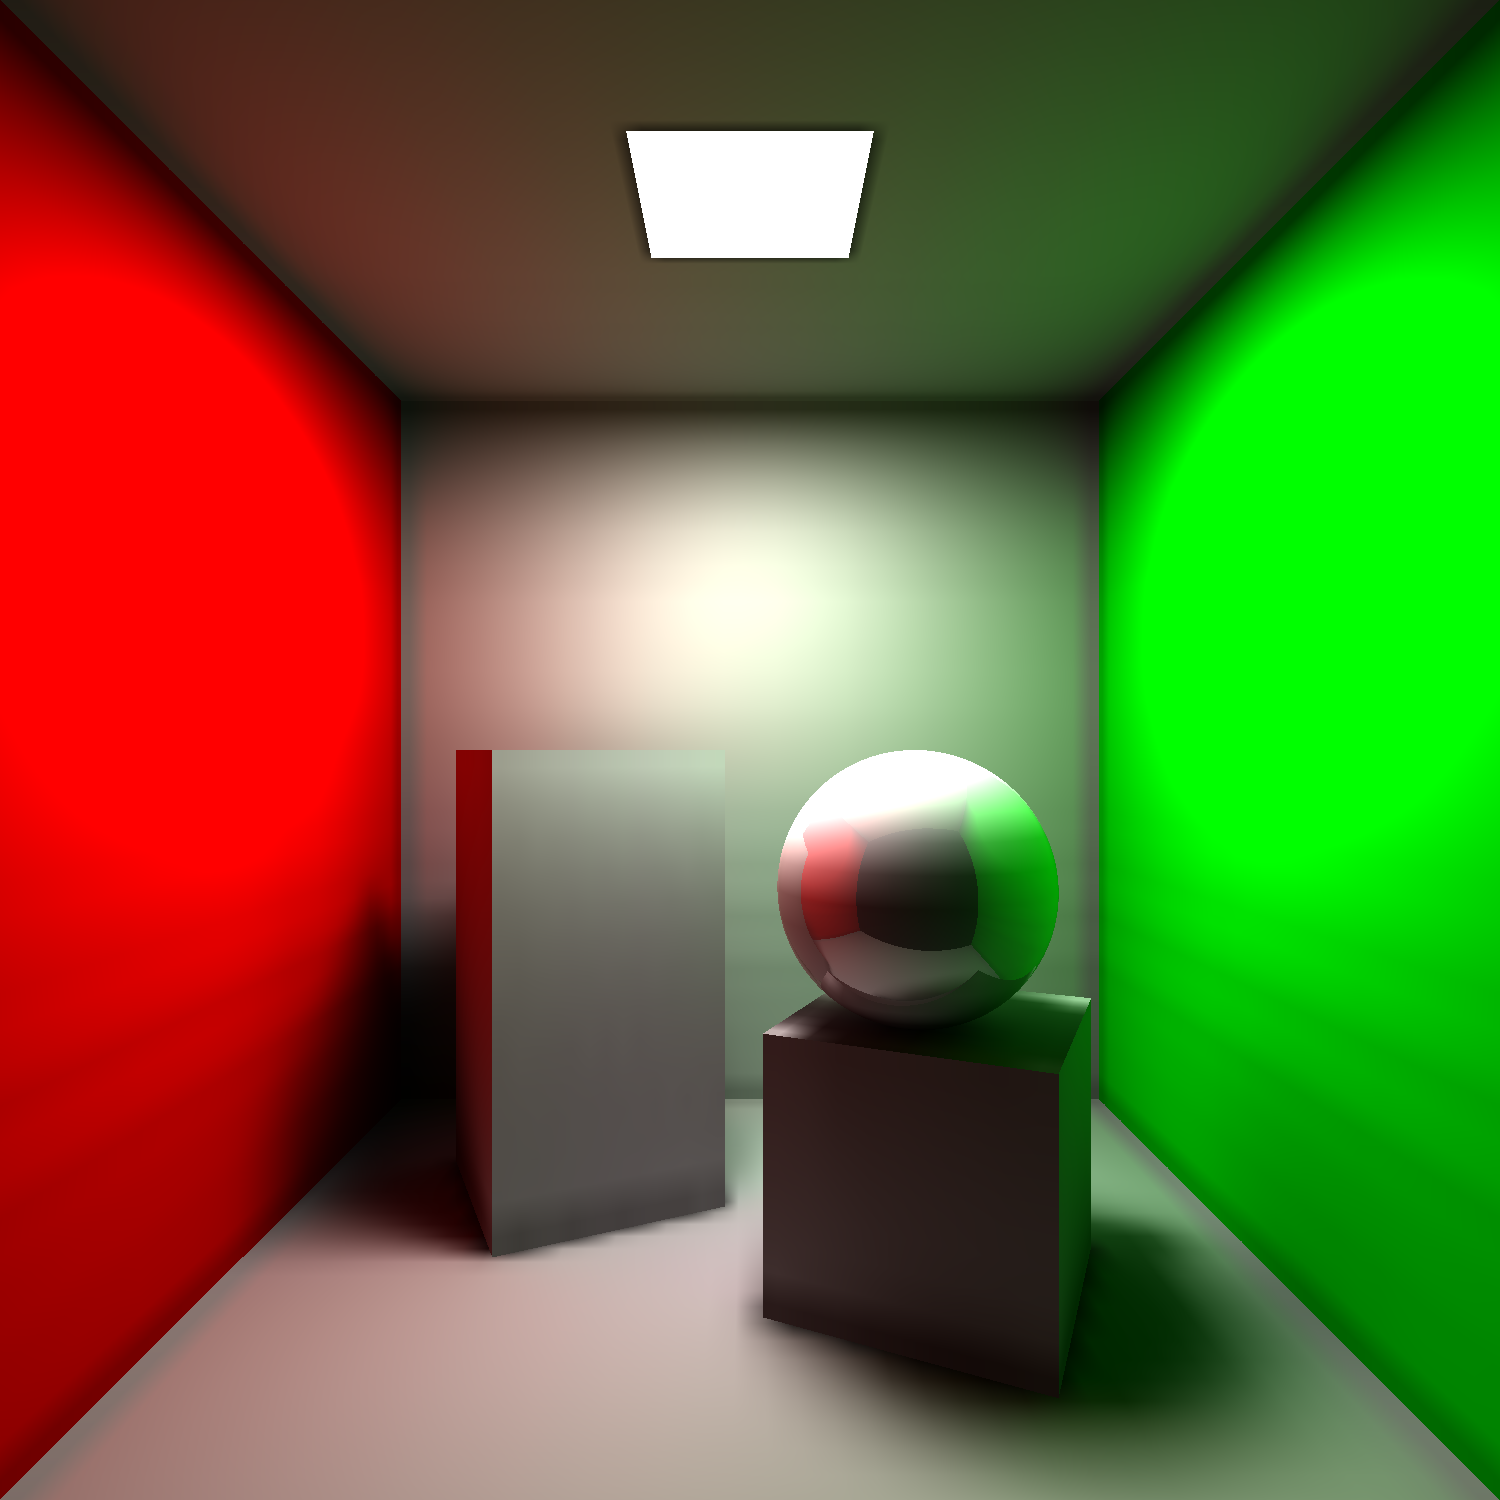
\includegraphics[width=6.0in]{reportfiles/teaser}
  \caption{Radiosity with specular effects.}
\end{teaserfigure}

\maketitle

\section{Introduction}

Our previous ray tracers were able to handle specular effects well, however suffered from an overly simplistic diffuse lighting model. Radiosity, in contrast, is capable of accurately modelling diffuse lighting, but cannot handle specular effects. Thus, to enhance our ray tracer, I implemented radiosity as the backend for diffuse information, with ray tracing being used for specular effects.

The papers \textit{The Hemi-Cube; A Radiosity Solution For Complex Environments} \cite{hemicube} and \textit{A Progressive Refinement Approach to Fast Radiosity Image Generation} \cite{progref} were used extensively to achieve fast performance in complex scenes enabling the simulation of thousands of iterations in minutes.

\section{Implementation}

Initially I implemented radiosity independently of the ray tracer. The radiosity engine splits up the scene into small patches and then the radiosity equation is solved iteratively. After enough iterations have been executed (once the patch energy states are considered converged enough) for initial debugging I rendered the patch states using OpenGL. Afterwards, I gave the ray tracer access to the patches of the radiosity engine's scene. When the ray tracer needs to know the diffuse color of an intersected surface, it finds the patch it hit and computes the interpolated color.

\subsection{Patch Construction}

\begin{figure}[t]
    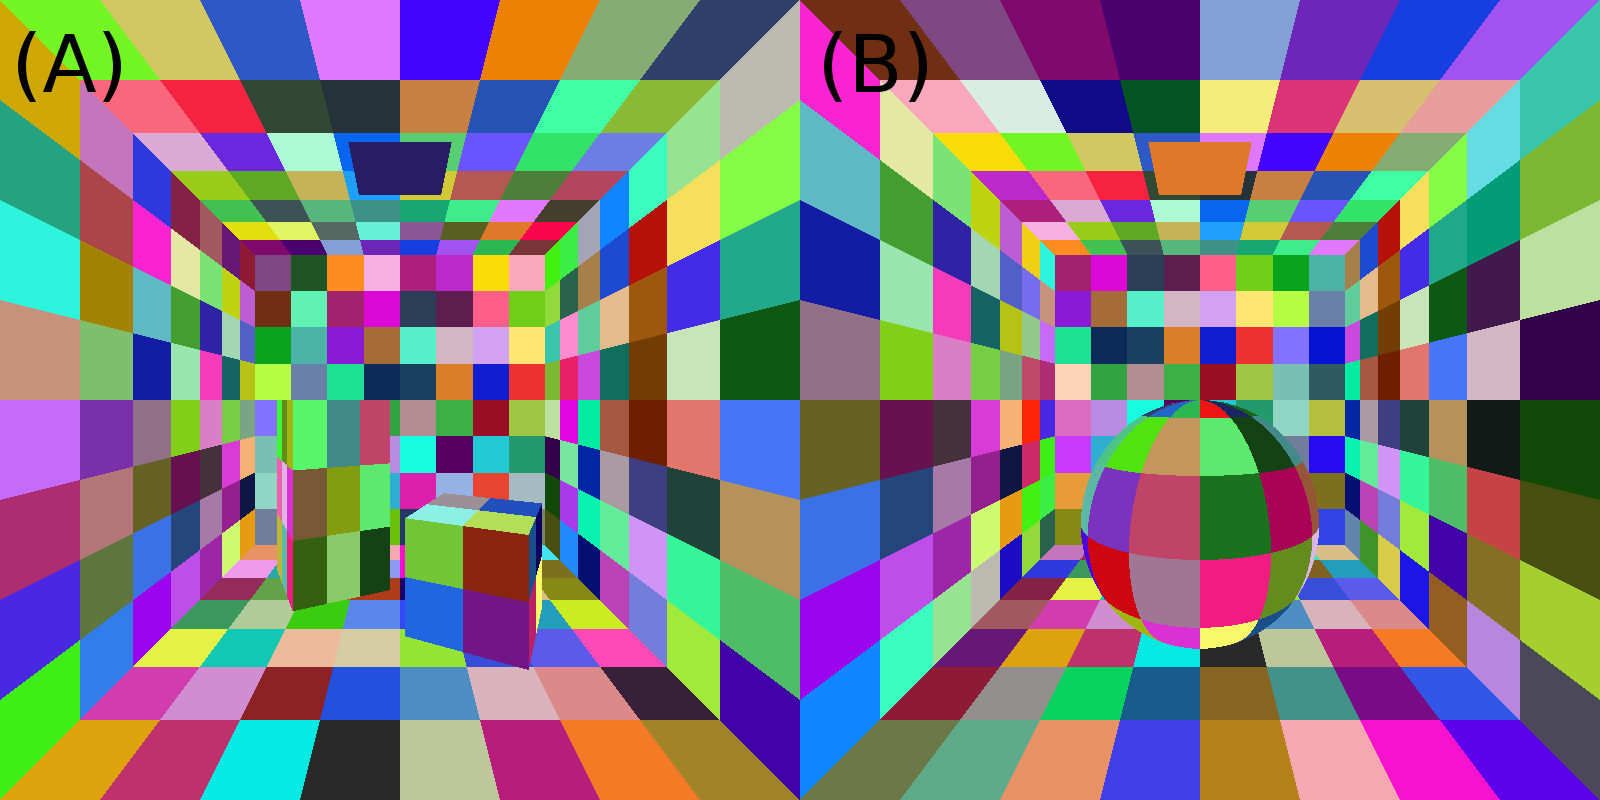
\includegraphics[width=\linewidth]{reportfiles/patches}
    \caption{(A) demonstrates the construction of patches on quads. (B) demonstrates the construction of patches on a curved surface (a sphere).}
    \label{fig:patches}
\end{figure}

First, the scene is broken up into individual patches, with each patch having a unique index, energy (color) value, and material (diffuse, emissive, specular). The user specifies a desired patch area (in units corresponding to the world coordinate system), and for each object in the scene the engine uses the surface UV coordinate system for that object to construct smaller patches. For quads, as demonstrated in diagram (A) of figure \ref{fig:patches}, the quad is broken up into smaller quad patches. For a desired patch area $A_d$ and a quad area $A$, the step size of the u, v coordinates $\Delta u$ and $\Delta v$ is given by:

\[\Delta u = \Delta v = \sqrt{A_d/A}\]

Additionally, the radiosity engine handles spheres. For spheres, as shown in diagram (B) of figure \ref{fig:patches}, curved patches are constructed. For a patch on a sphere of radius $R$, its length in the u direction $L_u$ and its length in the v direction $L_v$ is used to approximate the patch area with $A = L_u L_v$. From this the step size is approximated by:

\[\Delta u = \frac{1}{\pi} \arcsin{\frac{\sqrt{A_d}}{2 R}}\]
\[\Delta v = \frac{2}{\pi} \arcsin{\frac{\sqrt{A_d}}{2 R}}\]

Once the patches are constructed, their vertices are rendered to an OpenGL vertex buffer such that each vertex contains the world position and patch index. This buffer is used later for computing form factors.

\subsection{Solving the Radiosity Equation}

My implementation solves the radiosity equation using the progressive refinement approach \cite{progref}. Each patch $i$ in the scene has an amount of ``unshot energy'' $u_i$. When the scene is first constructed, $u B_i$ is the initial emitted light. 

Every iteration, the patch $i$ with the most unshot energy is selected and its form factors are calculated (the calculation is discussed in the next section). The patch $i$ then "shoots" its unshot energy to the other patches. Each patch $j$ is iterated over and its energy and unshot energy is updated:

\[ \Delta B_j = {\rho}_j u_i F_{ij} A_i/A_j\]
\[u_j' = u_j + \Delta B_j\]
\[B_j' = B_j + \Delta B_j\]

for diffuse reflectivity (i.e. "diffuse color") ${\rho}$, area $A$, and form factor from patch $i$ to $j$ is $F_{ij}$ \cite{progref}. After the energy from patch $i$ is shot, its unshot energy is reset by

\[u_i' = u_i F_{ii}\]

Every iteration the maximum unshot energy decreases. Iterations are performed until convergence is satisfactory.

\subsection{Form Factor Calculation}

\begin{figure}[t]
    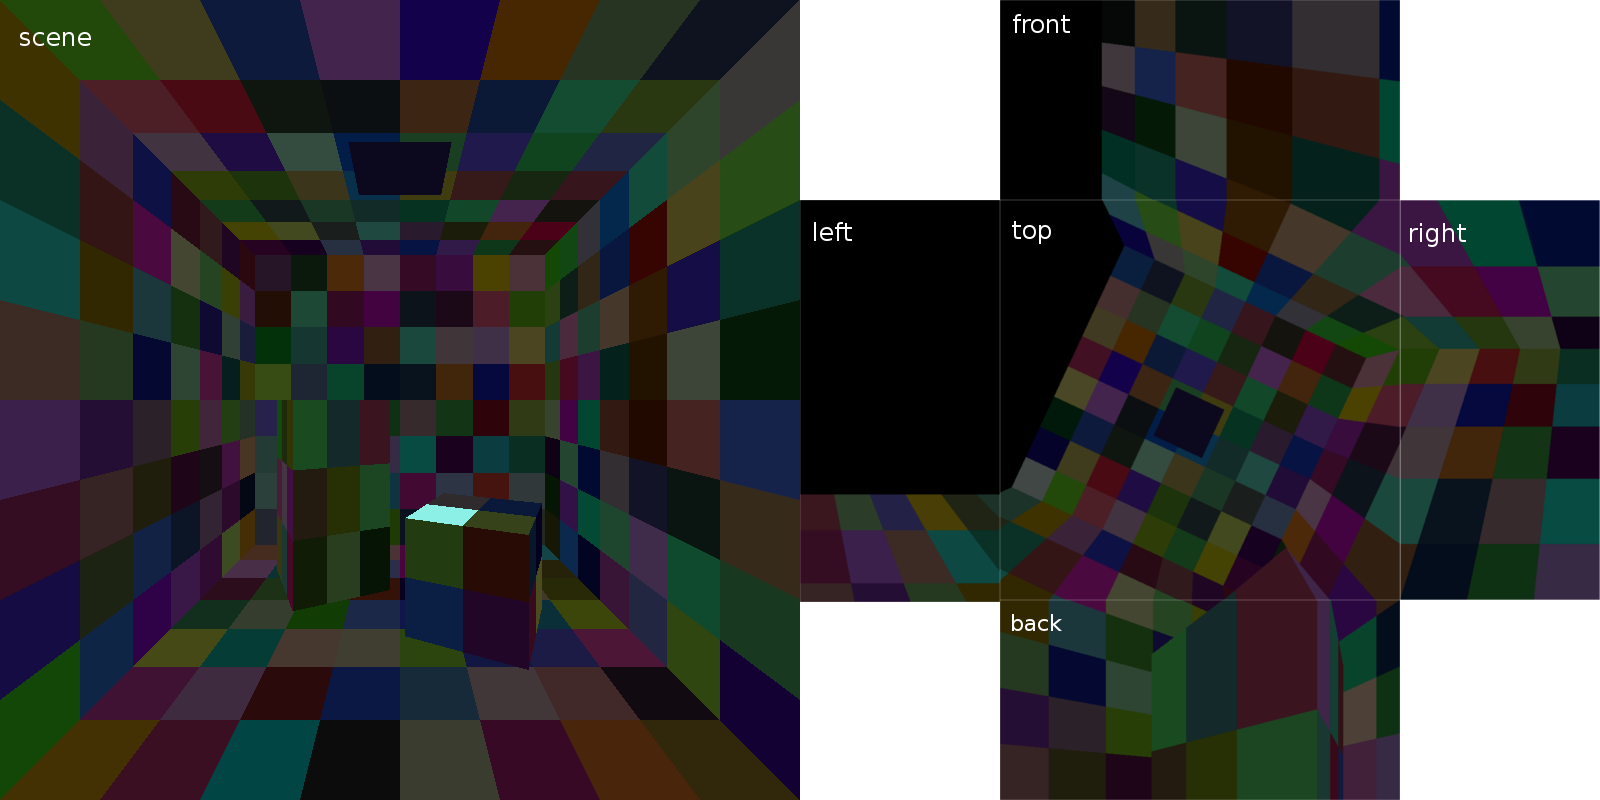
\includegraphics[width=\linewidth]{reportfiles/hemicube}
    \caption{The hemicube face renders for the highlighted patch.}
    \label{fig:hemicube}
\end{figure}

In order to compute $F_{ij}$ for a shooting patch $i$ the hemicube technique \cite{hemicube} is used. When the shooter patch is selected, an imaginary hemi-cube of height 1 is constructed around the center of the patch. As visualized in figure \ref{fig:hemicube}, the five faces of the hemicube are rendered quickly with OpenGL using a look-at matrix and a perspective transform with an FOV of 90 degrees. For each face, the resulting texture is a 2D array of patch indices. To compute the form factors, we iterate over texture's pixels: at a given pixel $(s, t)$ with patch index $j$ on a texture with dimensions $N_x \times N_y$, we compute $\Delta F_{ij}$:
\[x = 2 \frac{i}{N_x} - 1\]
\[y = 2 \frac{j}{N_y} - 1\]
\[{dA} = \frac{4}{N_x N_y}\]
\[
   \Delta F_{ij} = \begin{cases}
        \frac{{dA}}{x^2 + y^2 + 1} & \text{face is the top face} \\
        \frac{y {dA}}{x^2 + y^2 + 1} & \text{face is a side face}
   \end{cases}
\]

The $\Delta F_{ij}$ is then added to the form factor for patch $j$. After iterating over all five faces, the form factors from patch $i$ to all patches is known.

\subsection{Combining Radiosity with Ray Tracing}

\begin{figure}[t]
    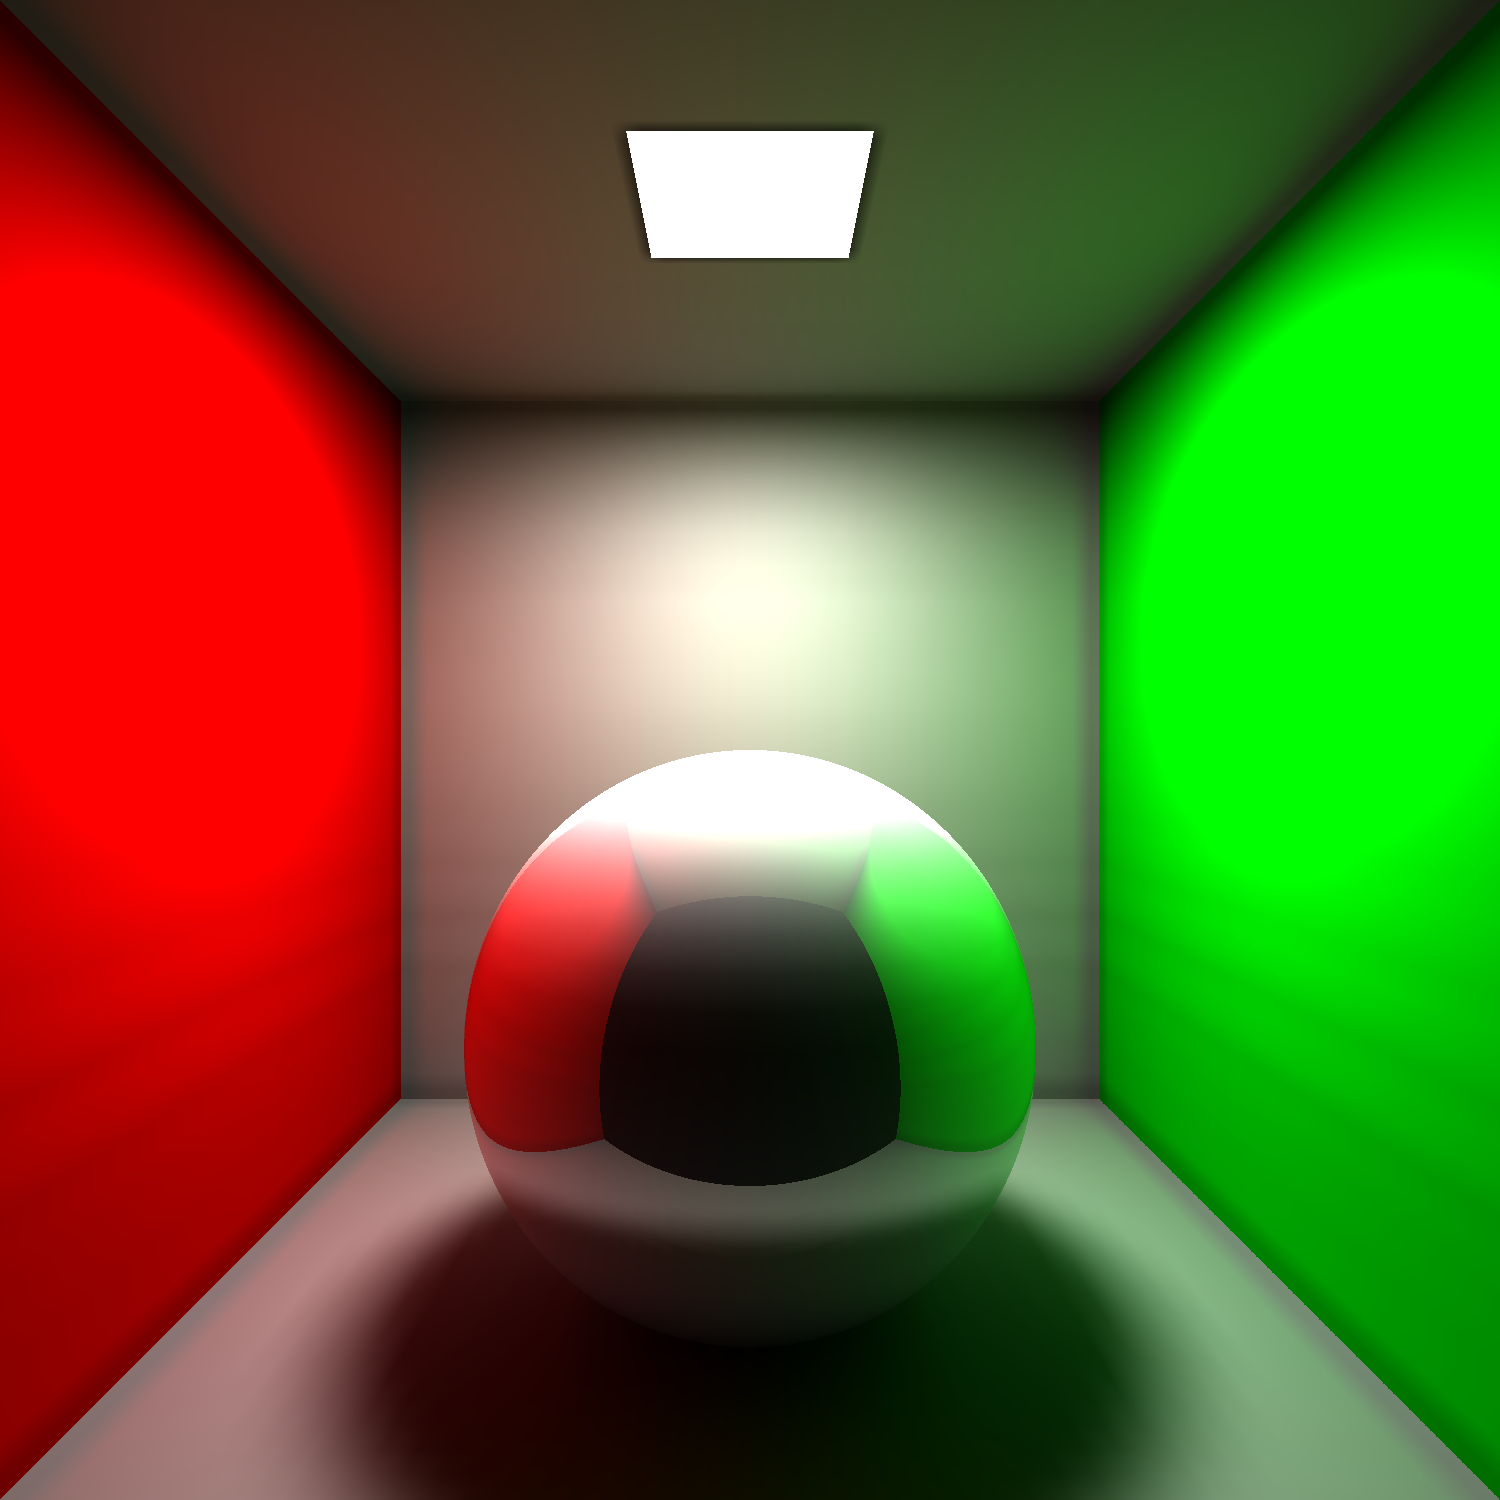
\includegraphics[width=\linewidth]{reportfiles/specular}
    \caption{Specular effects on the sphere with raytracing.}
    \label{fig:specular}
\end{figure}

In order to achieve specular effects with radiosity, the patches in the radiosity scene are used as the backend for diffuse colors. For a given object in the scene, its patches are placed in a 2D array with dimensions $N_u \times N_v$ such that when a ray intersects the object at surface coordinates $(u, v)$, the patch indices in the array can be computed with:

\[
    i = \lfloor u*N_u - 0.5 \rfloor
    j = \lfloor v*N_v - 0.5 \rfloor
\]

At these coordinates billinear interpolation is performed and the patch color is used as the diffuse color. If the surface is specular then a ray is reflected off the surface and its resulting color is added to the color of the surface.

Figure \ref{fig:specular} demonstrates the use of ray-tracing with radiosity.

\subsection{Material Shaders}

\begin{figure}[t]
    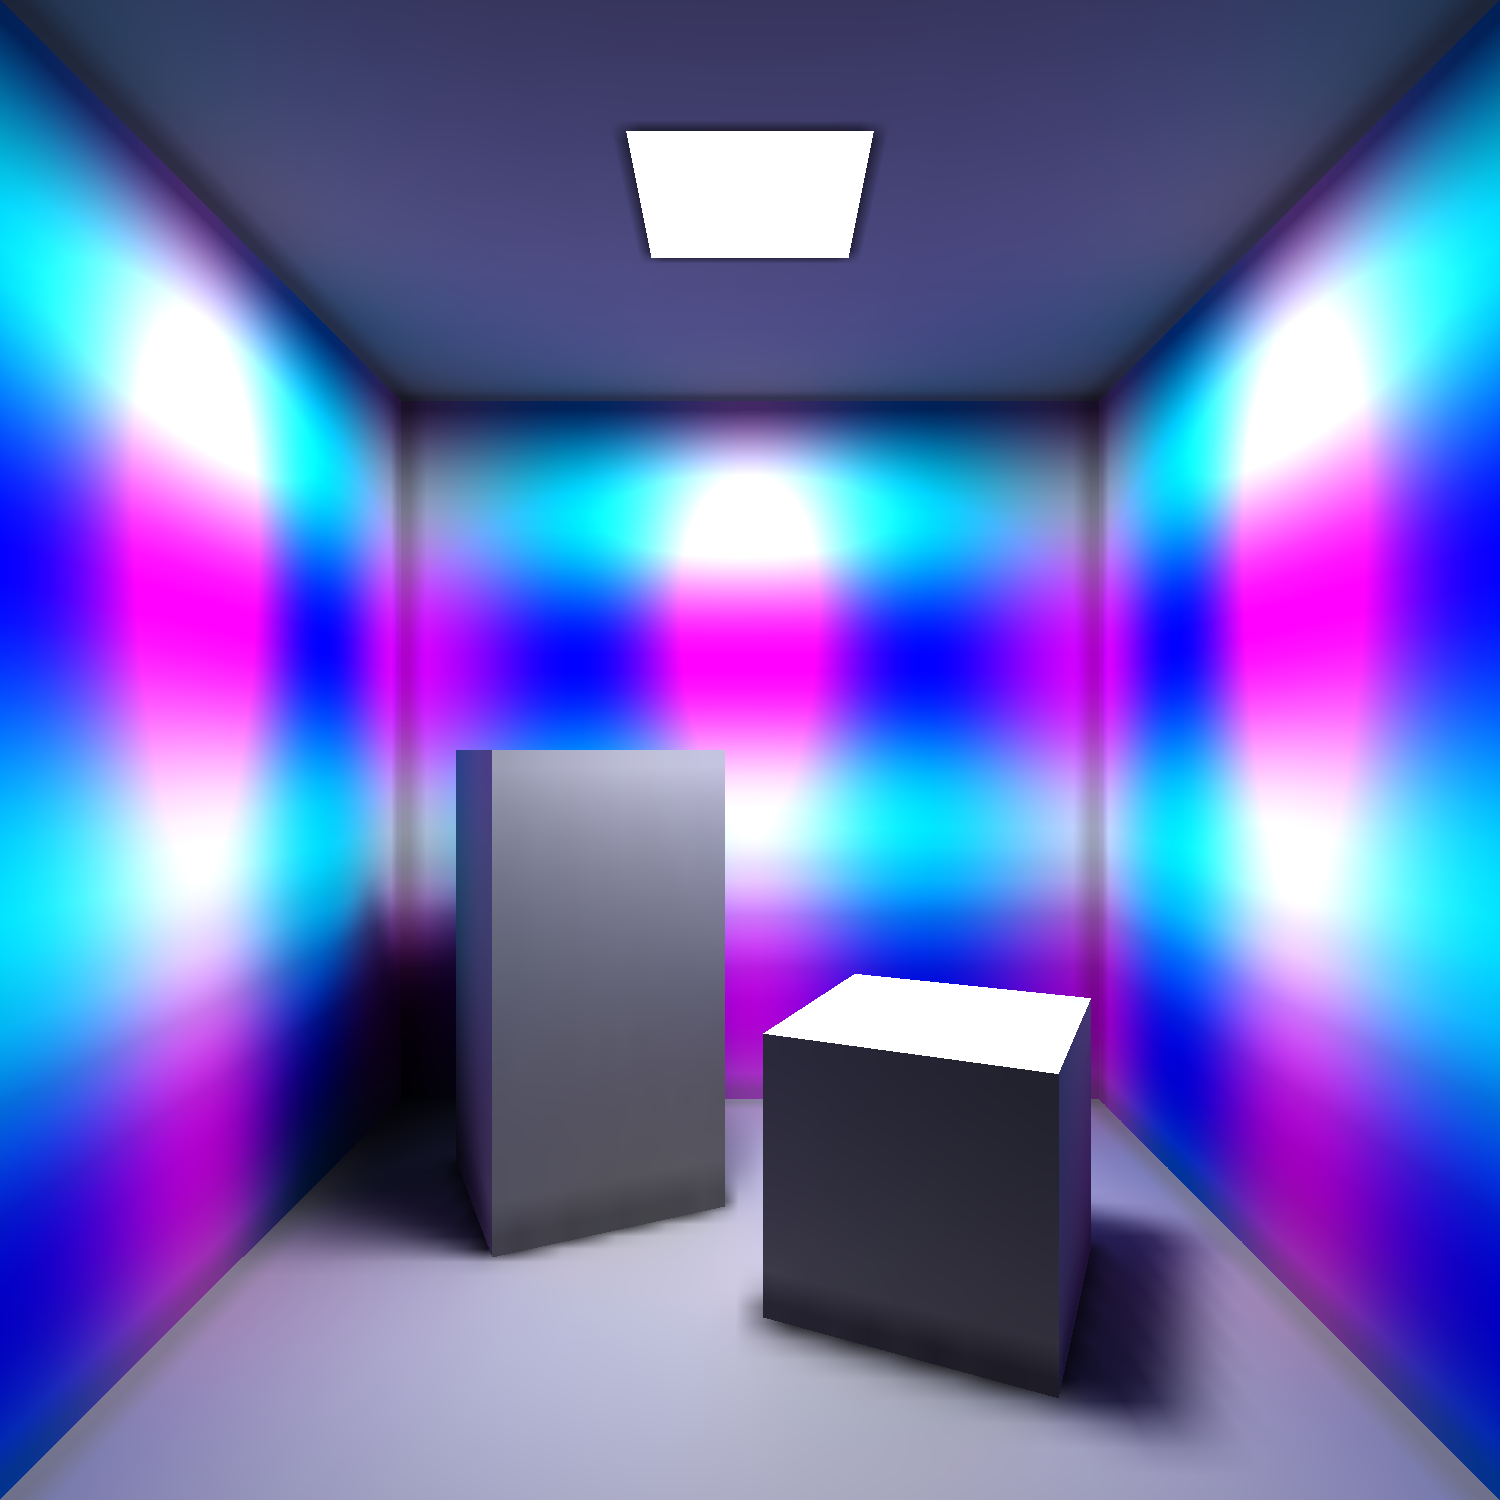
\includegraphics[width=\linewidth]{reportfiles/shaders}
    \caption{Material shaders on the walls.}
    \label{fig:shaders}
\end{figure}

Material shaders can be implemented in radiosity. In order to implement support for the material shaders like in our previous ray-tracer assignment, when constructing patches each patch normal and UV is used to parametrize the material shader. This works as long as the patch density is sufficiently high.

\section{Conclusion}

Radiosity can be used effectively to better model diffuse effects, and ray tracing can complement it to introduce specular effects. However, radiosity can be expensive, as a high patch density is required to eliminate artifacts from interpolation, and radiosity cannot handle sharp edges very effectively.

\bibliographystyle{ACM-Reference-Format}
\bibliography{report}
\end{document}
